% preamble:
\documentclass[12pt]{article}
\usepackage{amsmath,xcolor,todonotes,graphicx,marvosym,dsfont,import,fullpage,textcomp,colortbl,array,pgfplots,lscape}
\definecolor{grey}{gray}{0.5}
\definecolor{lightgrey}{gray}{0.8}
\usepackage[numbers]{natbib}
%\usepackage[papersize={85cm,30cm},left=2cm,top=2cm]{geometry}
%\usepackage[a3paper,left=2cm,top=4cm,bottom=4cm]{geometry}

%if you are annoyed of the colored boxes the hyperlinks in the pdf file uncomment this instead of the plain hyperref package above:
\usepackage[colorlinks=true, linkcolor=black, citecolor=black, urlcolor=black]{hyperref} 
\usepackage{NVC} %calles the style package NVC.sty created by Loes and Evert

%title infos
\date{\today}
\title{{\Huge Genetic Algorithm in the NVU}\\
	\vspace{2cm}
	Documentation of parameter optimization by using a Genetic Algorithm\\
	{\large BLABLABLABLABLABLA.
		\vspace{7cm}}}

\author{by Eva Waldhauser\footnote{University of applied Sciences Regensburg,  \href{mailto:eva.waldhauser@st.oth-regensburg.de}{eva.waldhauser@st.oth-regensburg.de}} $~$ \& Moritz Burger\footnote{University of applied Sciences Regensburg,  \href{mailto:moritz.burger@st.oth-regensburg.de}{moritz.burger@st.oth-regensburg.de}} }

%MATLAB code 
\usepackage[framed,numbered,autolinebreaks,useliterate]{mcode}

%Glossary
%\usepackage[
%nonumberlist, %do not show page numbers
%acronym,      %generate acronym listing
%toc,          %show listings as entries in table of contents
%section]      %use section level for toc entries
\usepackage{datatool}
\usepackage{glossaries}
\usepackage{hyperref}
\newglossary[slg]{symbolslist}{syi}{syg}{List of symbols} %Generate a list of symboles
\renewcommand*{\glspostdescription}{} %Remove the dot at the end of glossary descriptions
\makeglossaries %Activate glossary commands
\usepackage{glossary}

\pgfplotsset{compat=1.8}

%actual document:
\begin{document}
	\maketitle
	\newpage
	\tableofcontents
	\thispagestyle{empty}
	\newlength\figureheight
	\newlength\figurewidth
	
	\section{Introduction}
\subsection{Neurovascular Unit}
%what cells do we look at and how are they orientated to each other? - take parts of L\&E

The cerebral cortex, a highly complex component of the human brain and part of the grey matter (\textit{substantia grisea}),   mainly consists of neurons (\gls{NE}s), unmyelinated axons and glial cells such as astrocytes (\gls{AC}s). It forms the outer layer of \textit{cerebrum} and \textit{cerebellum} and is veined with capillary blood vessels that provide the brain tissue with glucose and oxygen (\citet{Shipp2007}). These arterioles are surrounded by endothelial cells (\gls{EC}s) that form a thin layer on the interior surface of arterioles (\textit{intima}). The outer layer of the arteriole consists of smooth muscle cells (\gls{SMC}s), which are  aligned in circumferential direction. They define the contractile unit of the vessel and regulate its diameter by contraction and dilation.\\

A neurovascular unit (\gls{NVU}) defined in this research includes one cell of each of the described types and is graphically pictured in Figure~\ref{Overview1}. \\ 
\begin{figure}[h!]
  \centering
  \def\svgwidth{450pt}
  \scriptsize 
%  \includegraphics[width=130mm]{Bilder/Overview_NVU.png}
  \import{pics/}{Overview_without_gaps.pdf_tex}
  \caption{\textbf{Overview of different cells and domains that form a neurovascular unit.}  \gls{NE} - Neuron, \gls{SC} - Synaptic Cleft, \gls{AC}  - Astrocyte,  \gls{ER}  - Endoplasmic Reticulum,  \gls{PVS}  - Perivascular Space,  \gls{SMC}  - Smooth Muscle Cell, SR - Sarcoplasmic Reticulum,  \gls{EC}  - Endothelial Cell,     \gls{LU}  - Lumen with indicated blood flow. Intercellular communication via the exchange of ions is indicated by arrows. }
\label{Overview1}
\end{figure}

Each of the cell types and the spaces in between play an important role within the process of neurovascular coupling (\gls{NVC}, see Section \ref{section:NVC}). The synaptic cleft (\gls{SC}) is the space between an axon terminal and dendrite of two different \gls{NE}s in which neurotransmitters are released. It is enclosed by the star-shaped \gls{AC} that can take up released neurotransmitters. Protoplasmic \gls{AC}s are  polarized cells which can temporarily buffer extracellular \gls{K}, which is one of the key mechanisms within \gls{NVC}.  The astrocytic endoplasmatic reticulum (\gls{ER}), an isolated space in the cytosol, contains \gls{IP3}-sensitive \gls{Ca} channels, which can release \gls{Ca}-ions into the cytosol. The perivascular space (\gls{PVS}) is located between the end feet of an \gls{AC} and the arteriole. In the \gls{PVS}, ion exchange occurs between the arterial wall and the \gls{AC}.  The \gls{EC}s form a monolayer on the luminal side of the vessel in which all cells are aligned in the direction of the flow. It prevents passive diffusion of bigger molecules, while small ones, such as \gls{O2}, \gls{Ca} or \gls{IP3}, can pass through.  It also functions as an active organ sensing wall shear stress which plays an important role in the \gls{NO}-mediated pathway. Together with the SMC layer the endothelium forms the blood brain barrier (BBB), the physical frontier between brain tissue and blood vessel.
\gls{SMC} contraction occurs by actin and myosin filaments forming cross-bridges. The rate of contraction is dependent on the \gls{SMC} cytosolic \gls{Ca} concentration.
 






\subsection{Neurovascular Coupling} \label{section:NVC}
Neurovascular coupling (\gls{NVC}), or functional hyperaemia, describes the local vasodilation and~-contraction due to neuronal activation. The change in the vessel diameter (vasoreactivity) controls the blood flow and thereby the cerebral supply of oxygen and glucose.

Each cell type plays an important specific role during the process of NVC. Communication between cells is based on an exchange of ions through pumps and channels. These ion fluxes contribute to changes in cytosolic and intercellular species concentration and cell membrane potentials.

There are several pathways that can lead to vasocontraction or -dilation and are mediated by different signalling molecules, such as \gls{K}, \gls{Ca}, EET, \gls{NO} and 20-HETE. Neurotransmitters are released by the \gls{NE} into the \gls{SC} and can bind to receptors on dendrites of other neurons and astrocytes. This leads to a cascade of chemical reactions and the opening and closing of ion channels which influences the fluxes and concentrations.

%
%  be taken up by
%
% of events finally leading to inositol trisphosphate (IP3) production in the astrocytic cytosol [24].
% 
% 
% %  
%A change in the astrocyte’s membrane potential together with the increased EET concentration activates the BK-channels. These channels are located on the end-feet of the astrocyte and cause an efflux of K+ ions into the perivascular space. During neuronal activation this efflux increases.
%A moderate increase in the potassium concentration in the perivascular space causes the activa- tion of the potassium inward rectifying (KIR) channel. This KIR channel causes a depolarisation of the SMC. However, when the perivascular space’ potassium concentration is increased above a certain level, the KIR channel starts pumping potassium out of the cell, causing hyperpolarisation [2, 12].
%The voltage operated calcium channel (VOCC), which also interacts between SMC and its extra cellular space, pumps calcium into the cytosol. The influx of Ca2+ ions through the VOCC decreases when the SMC hyperpolarises [29] and amplifies the hyperpolarisation of the SMC.
%This hyperpolarasition decreases the influx of calcium. The calcium concentration in the SMC influences the myosin binding process. Actin filaments have several binding sites to which myosin can bind. However, in rest these binding sites are blocked by troponin. Free Ca2+ ions will cause troponin to move slightly which opens the binding sites. Then, cross bridges can be made between the actin and myosin. During hyperpolarisation, fewer Ca2+ ions enter the SMC. Consequentially, fewer cross bridges can be formed, which means that the vessel will dilate.
%A dilated vessel decreases the resistance to the flow, which causes an increase of flow and decrease of pressure drop over the vessel. Higher blood flow increases the diffusion process of chemicals, for example oxygen, through the cell wall into the surrounding tissue. Note that this is the intended response to neuronal activation of the NVU.
%
%%This document describes the code which includes the models of Ostby, Koenigsberger, HaiMurphy 


\subsection{Mathematical Approach}
The physiological models are based on a set of differential equations that describe the mass conservation of ions and molecules passing from one cell or domain to another. The simulations describe time-dependent ion fluxes and changes in membrane potential modelled by reaction rates that describe the kinetics which are physiologically validated by experimental data from the literature. This approach assumes homogeneous behaviour of a variable in a certain subdomain i.e. the spatial gradient of a variable in every subdomain is negligible.
%general mathematical modelling - definition of domains ('boxes') -  In the models  a lumped parameter approach is used.
%cells communicate with each other via ion fluxes - mathematically, this communication can be expressed by differential equations describing the mass conservation (explain!) and changes in membrane potential  

 



	hallo 
	hallo
	%\documentclass[12pt]{article}
%\usepackage{amsmath,xcolor,todonotes,graphicx,marvosym,dsfont,import,fullpage,textcomp,colortbl,array,pgfplots,lscape}
%\begin{document}
	\section{Results}
	\subsection {OO-NVU 2.0}
	\subsubsection*{Potassium input signal (figure \ref{fig:1IS})}
	At the top the neuronal \gls{K} input signal is shown. This input signal is pumped into the SC by the \gls{NE}. As a result of that, there is more \gls{K} taken up by the \gls{AC} in the beginning of the input pulse, and released at the end of the input pulse. In the second graph the membrane potential of the AC is shown over time. When the \gls{K} concentration in the SC is increased the membrane voltage depolarises and when the \gls{K} concentration in the SC decreases the membrane potential repolarises again.
	In the third graph the fluxes into the PVS are shown. In blue the flux by the astrocytic BK channel, and in green the flux by the KIR channel in the SMC is shown. The drop in the middle of the KIR flux is caused because the SMC becomes in a oscillatory state and therefore the efflux by the KIR channel follows the \gls{Ca} waves inside the SMC.
	The bottom figure shows the \gls{K} concentration in the PVS.
	
	\subsubsection*{Neurovascular Coupling Overview (figure \ref{fig:1})}
	This figure describes the main pathway from the synaptic cleft to the radius change. It starts with a \gls{K} concentration in the synaptic cleft, followed by the flux trough the BK-channel determined in the astrocyte, leading to an increased \gls{K} concentration in the perivascular space. This causes an increased  \gls{K} influx trough the KIR channel, changing the membrane voltage of the SMC. The \gls{Ca} flux through the VOCC increases, decreasing the \gls{Ca} concentration in the SMC and thereby inducing vasodilation. 
			
	
	\subsubsection*{AC State Variables (figure \ref{fig:2})}
	The graphs display the concentrations of \gls{K}, \gls{Ca}, Cl and HCO3 in the astrocyte and \gls{K} in the SC and PVS. These concentrations, together with the membrane voltage contribute to the opening of the BK-channel in their own way. The open state of the BK channel determines the potassium flux from the astrocyte to the perivascular spcace, where it induces vascular contraction.
	
	\subsubsection*{AC Fluxes (figure \ref{fig:3})}
	All ion fluxes that enter or leave the astrocyte.
	
	
	\subsubsection*{SMC EC State Variables and Coupling (figure \ref{fig:4})}
	The graphs in this figure shows the solutions of the differential equations of the \gls{SMC} and \gls{EC}, including the intracellular \gls{Ca} concentration, the \gls{IP3} concentration, the sarcoplasmic (\gls{SMC}) or endoplasmic (\gls{EC}) \gls{Ca} concentration, the membrane voltage and the coupling fluxes between EC and SMC.
	
	\subsubsection*{SMC Fluxes (figure \ref{fig:5})}
	In these figures the coupling and the fluxes in the SMC are shown. When one of the fluxes is negative, it means that the direction of the flux is in the opposite than it is defined in the equations. These figures show that when the neuronal signal is given, the VOCC closes and that the SMC contracts. 
	
	\subsubsection*{EC Fluxes (figure \ref{fig:6})}
	All ion fluxes that enter or leave the EC.
	
	\subsubsection*{Contraction Model and Radius (figure \ref{fig:7})}
	In this figure the fraction of the four states (M, Mp, AMp, AM) of myosin in the SMC are shown at the top. At the bottom left the fraction of attached cross bridged myosin (the sum of AM and AMp) is shown. And at the bottom right the radius is plotted over time. The increase in vessel diameter is in the expected order of magnitude.
	
	
	\begin{landscape}
			
		\begin{figure}[h!]
			\centering
			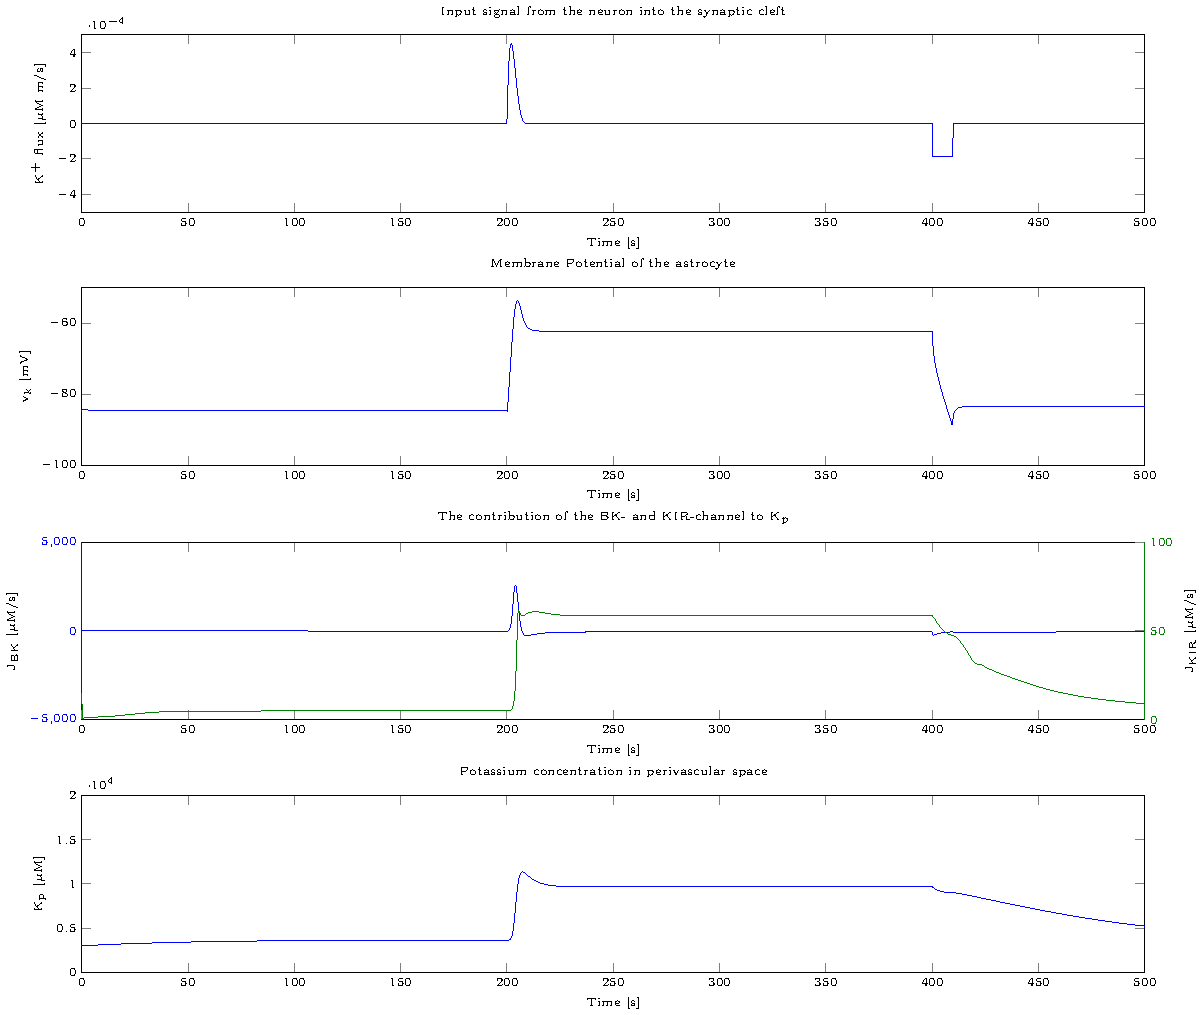
\includegraphics{figures/1_Input_signal.pdf}
			\caption{The input signal.}
			\label{fig:1IS}
		\end{figure}
		
		\begin{figure}[h!]
			\centering
			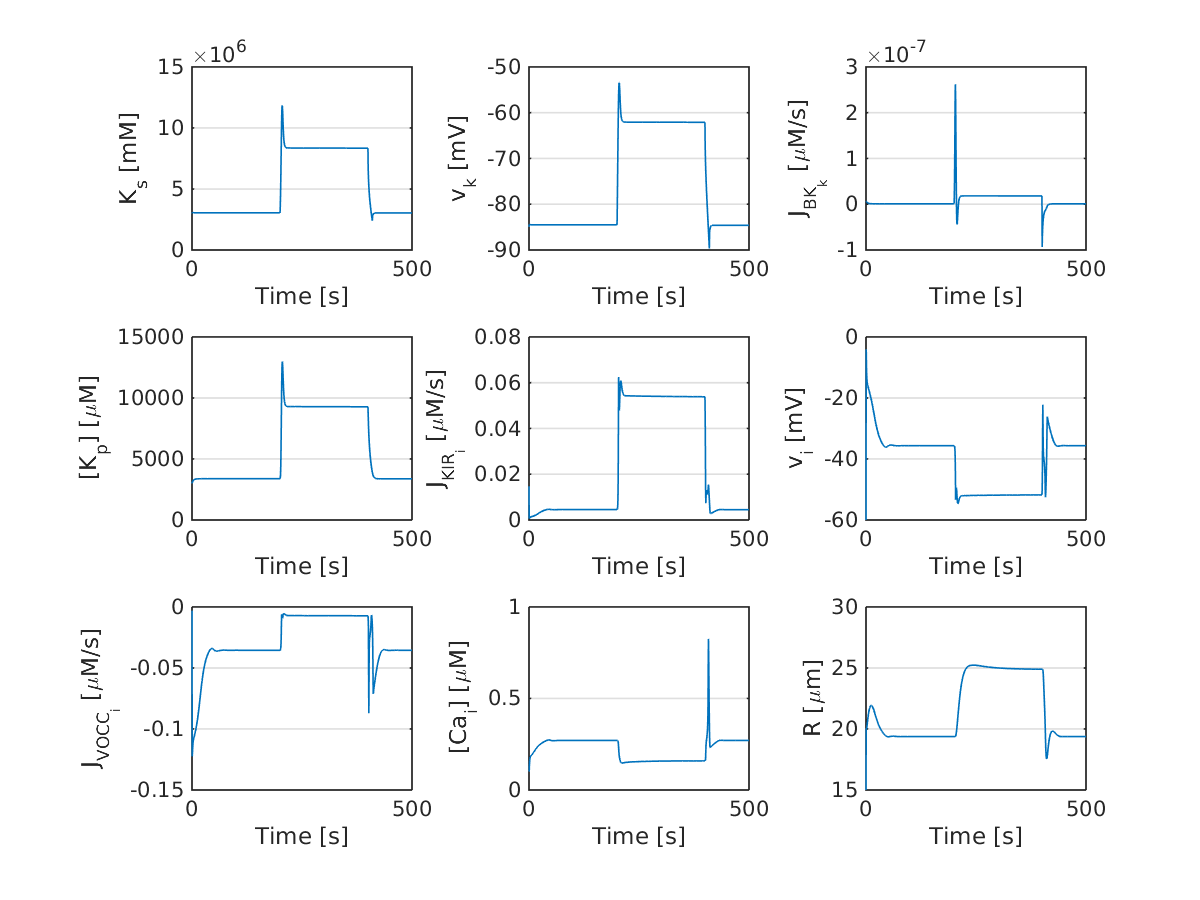
\includegraphics{new_figures/1 Neurovascular Coupling Overview.png}
			\caption{Neurovascular Coupling Overview.}
			\label{fig:1}
		\end{figure}		
		
		\begin{figure}[h!]
			\centering
			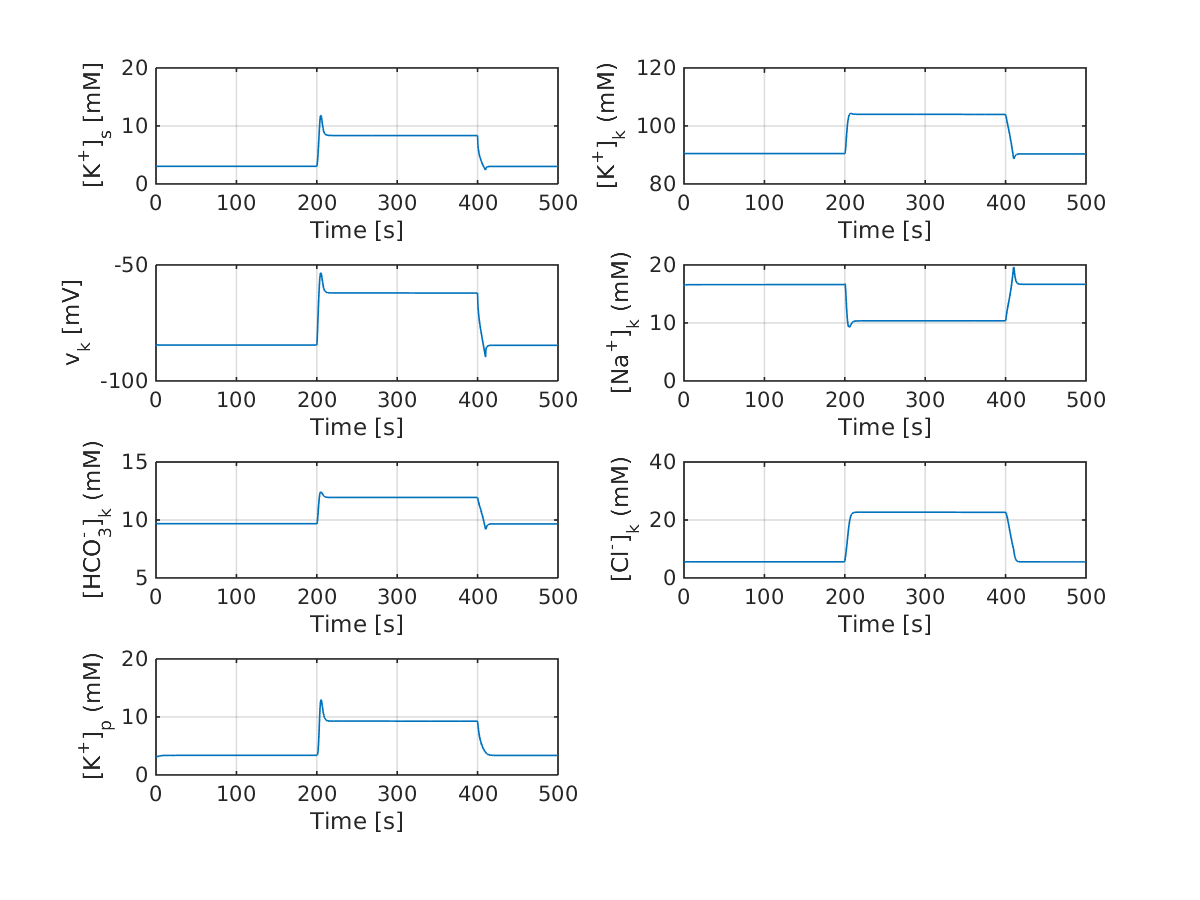
\includegraphics{new_figures/2 AC State Variables.png}
			\caption{AC State Variables.}
			\label{fig:2}
		\end{figure}
	
	
		\begin{figure}[h!]
			\centering
			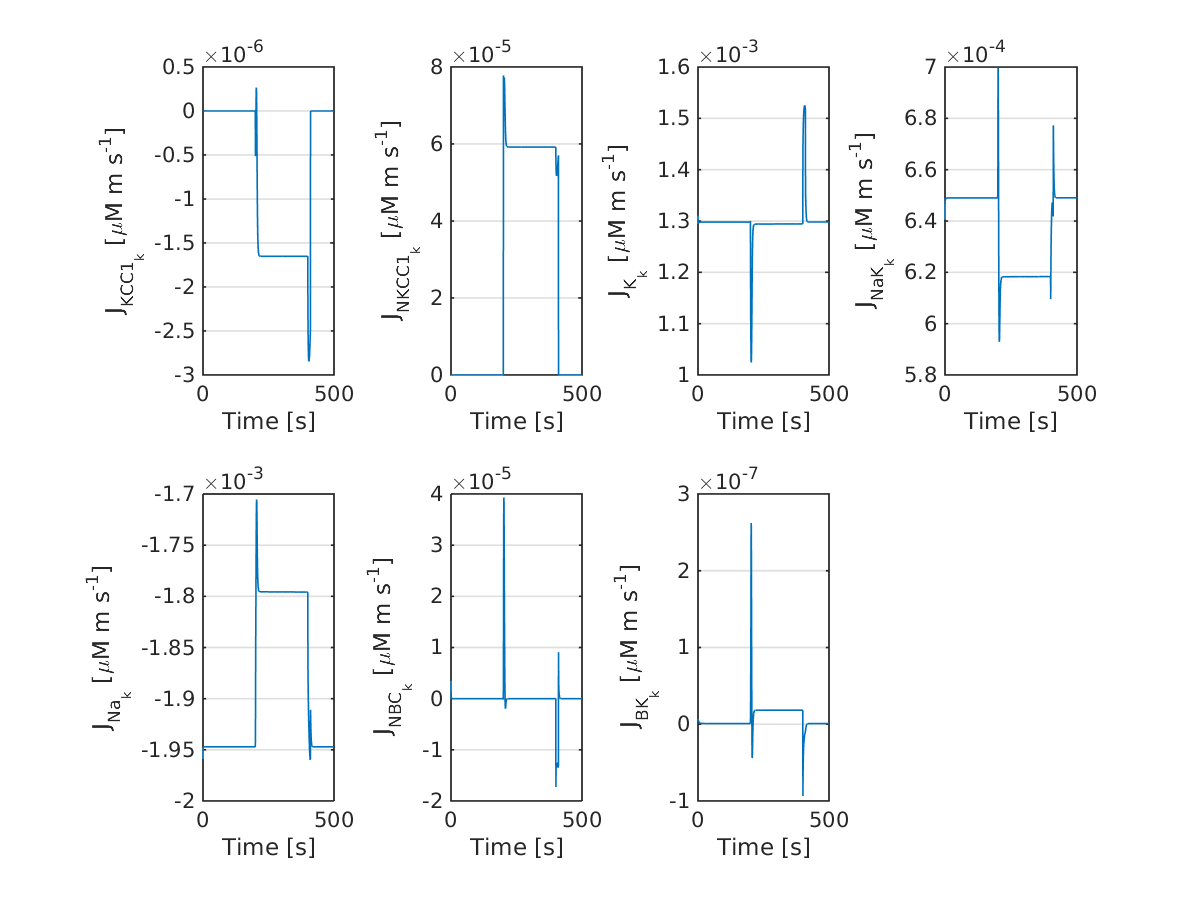
\includegraphics{new_figures/3 AC Fluxes.png}
			\caption{AC Fluxes.}
			\label{fig:3}
		\end{figure}
		
		
		\begin{figure}[h!]
			\centering
			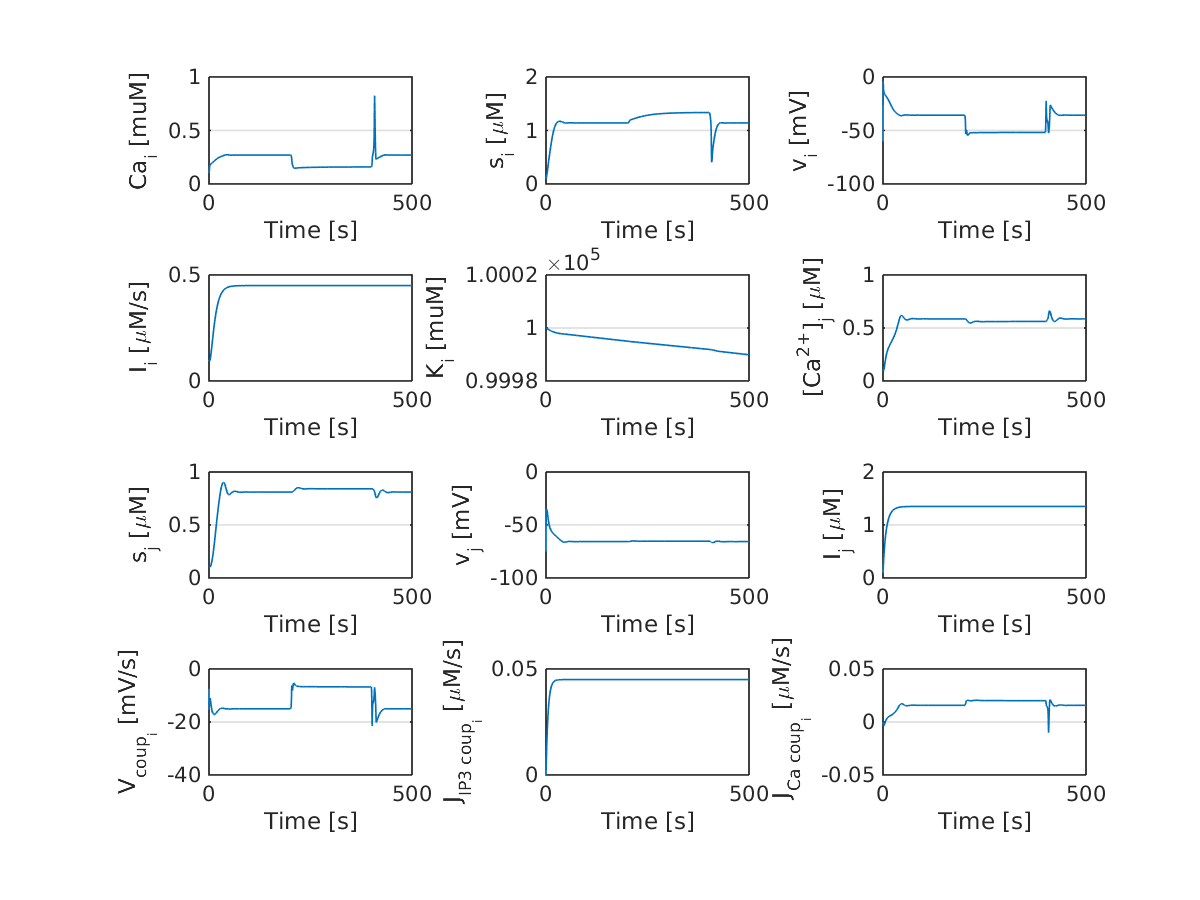
\includegraphics{new_figures/4 SMC EC State Variables and Coupling.png}
			\caption{SMC EC State Variables and Coupling.}
			\label{fig:4}
		\end{figure}
			
		\begin{figure}[h!]
			\centering
			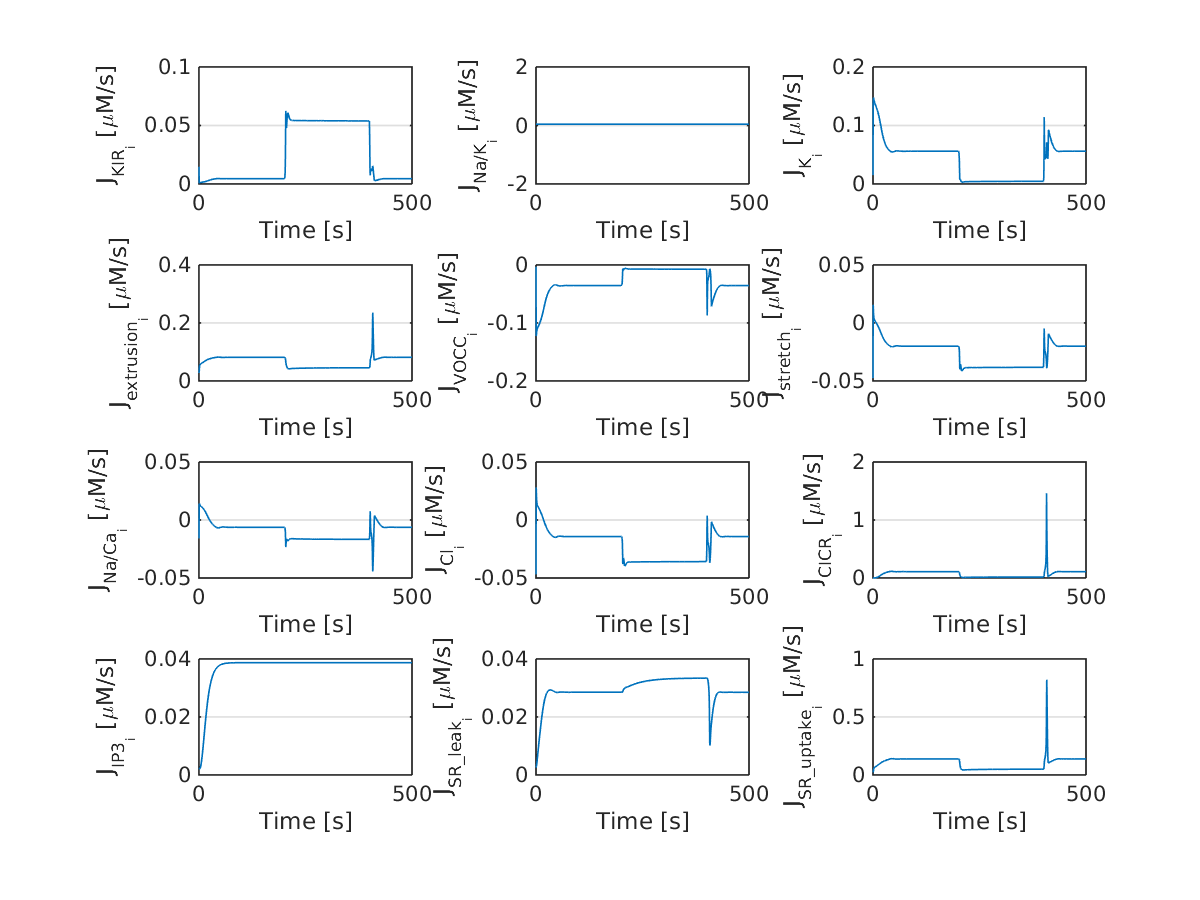
\includegraphics{new_figures/5 SMC Fluxes.png}
			\caption{SMC Fluxes.}
			\label{fig:5}
		\end{figure}
		
		\begin{figure}[h!]
			\centering
			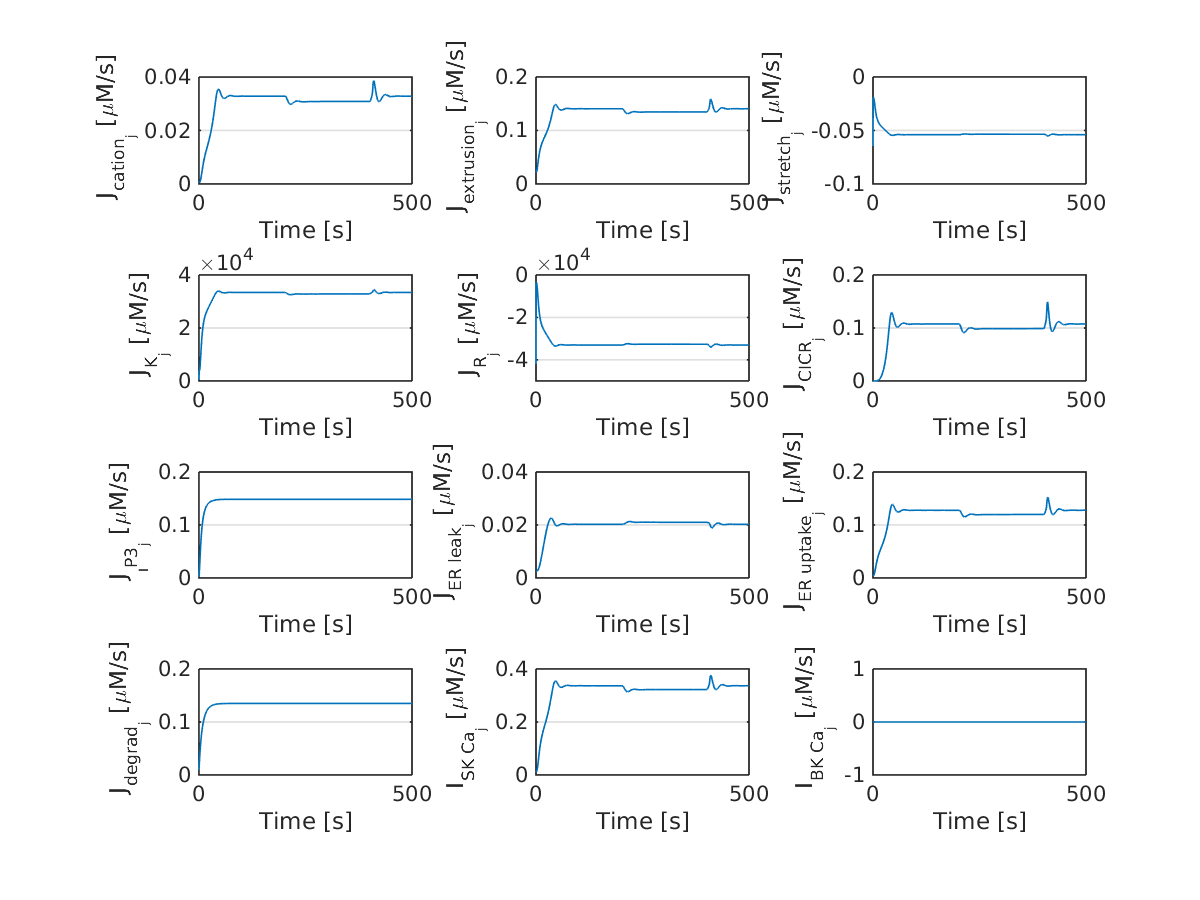
\includegraphics{new_figures/6 EC Fluxes.png}
			\caption{EC Fluxes.}
			\label{fig:6}
		\end{figure}
		
		\begin{figure}[h!]
			\centering
			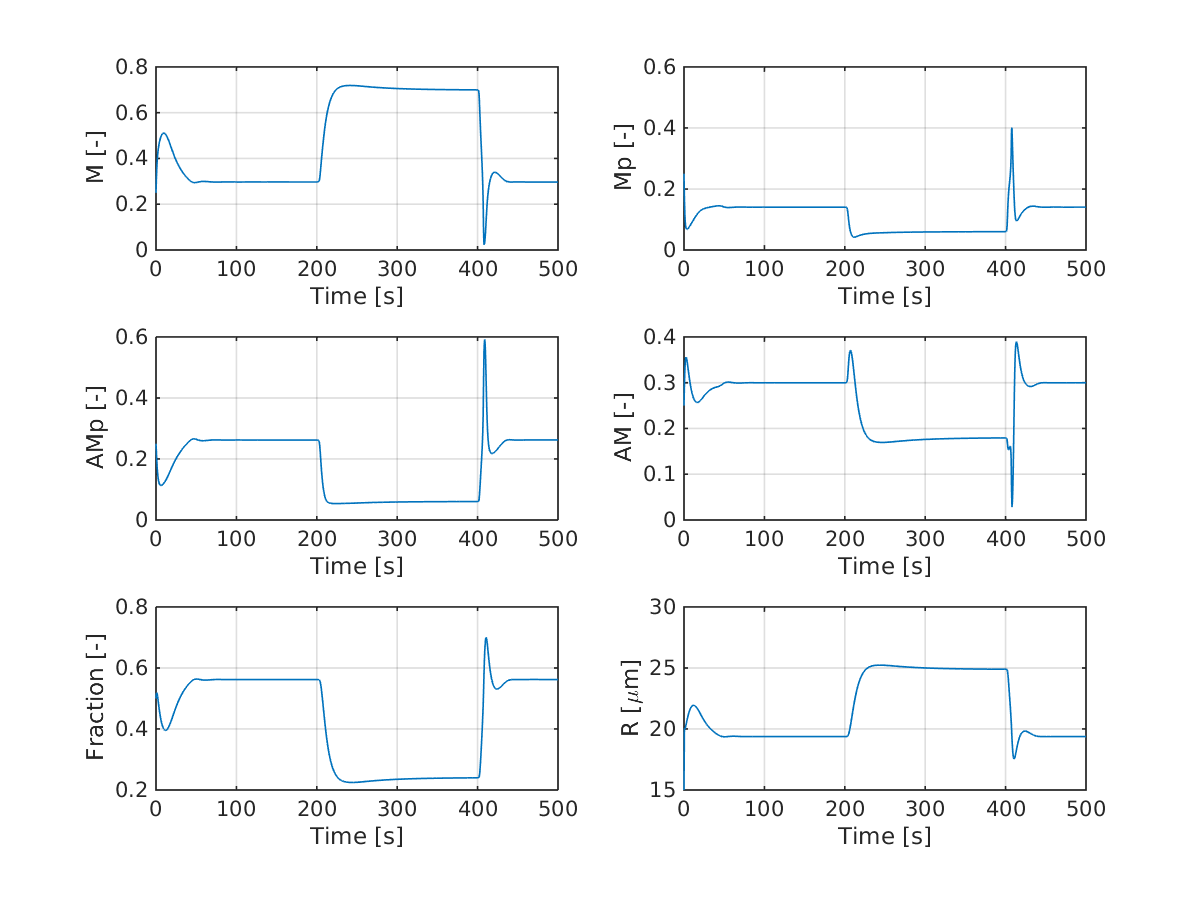
\includegraphics{new_figures/7 Contraction Model and Radius.png}
			\caption{Contraction Model and Radius.}
			\label{fig:7}
		\end{figure}
				
	\end{landscape}
	

	hallo

	
	%\nocite{*} % a good, but also very dangerous command! :) Shows all library entries
	
	\bibliography{library} %library.bib - any library file - either generated by Mendeley, Qiqqa, JabRef ... or write it your own, but don't complain if you choose to do so! :)
	\bibliographystyle{KathisBibstyle} % default: plain, ieeetr, named, acm, but there are many hp's where you can autogenerate your own Bibstyle! - or use mine for the start :)
	
	\newpage
	%\deftranslation[to=German]{Acronyms}{Abkürzungsverzeichnis}
	%\printglossary[type=\acronymtype,style=long]
	\printglossary[style=altlist,title=Glossary] %Print the glossary
	%\printglossary[type=\acronymtype,style=long] %Print list of acronyms
	
	%\section{MATLAB Code}

\subsection*{NVC\_main.m}
    \lstinputlisting[language=Matlab]{NVC_main.m}
\newpage
\subsection*{DEsyst.m}
    \lstinputlisting[language=Matlab]{DEsyst.m}
\newpage
\subsection*{all\_fluxes.m}
    \lstinputlisting[language=Matlab]{all_fluxes.m}
\newpage
\subsection*{writeFlux.m}
    \lstinputlisting[language=Matlab]{writeFlux.m}
\newpage
\subsection*{InitCond.m}
    \lstinputlisting[language=Matlab]{InitCond.m}
\newpage
\subsection*{all\_indices.m}
    \lstinputlisting[language=Matlab]{all_indices.m}
\newpage
\subsection*{all\_constants.m}
    \lstinputlisting[language=Matlab]{all_constants.m}
\newpage
\subsection*{createPulse.m}
    \lstinputlisting[language=Matlab]{createPulse.m}
\newpage
\subsection*{createSig.m}
    \lstinputlisting[language=Matlab]{createSig.m}
\newpage
\subsection*{getRef.m}
    \lstinputlisting[language=Matlab]{getRef.m}
\newpage
\subsection*{plot\_all.m}
    \lstinputlisting[language=Matlab]{plot_all.m}
\end{document}
